%%%%%%%%%%%%%%%%%%%%%%%%%%%%%%%%%%%%%%%%%%%%%%%%%%%%%%%%%%%%%%%%%%%%%%%%%%%%%%%

\chapter{PROPOSTA}
\label{ch:prop}

Nesta seção apresentamos os dados que serão utilizados e são relevantes para a operação, bem como apresentamos o fluxo de dados utilizado nos trabalhos correlatos e a arquitetura proposta, explicando o cubo de dados que será implementado.

\section{Dados}
\label{ch:prop:data}

A tabela \ref{table:bigdatasattypes} mostra os tipos de dados relevantes para a operação, a sua origem e o seu formato esperado, ignorando os dados provenientes da carga útil.

\begin{table}[!ht]
  \begin{center}
  \caption{Dados de Operação}
  \begin{tabular}{|c|C{5cm}|c|}
      \hline
      \bfseries Tipo de Dado &\bfseries Origem &\bfseries Formato \\
      \hline
      Sensores de bordo & Equipamentos no satélite & Tabelas, CSV \\
      \hline
	  Registros do Computador & Computador de Bordo & Texto (\textit{Logs}) \\
      \hline
	  Multimídia & Câmeras & MP4, JPG, RAW \\
      \hline
	  Parâmetros orbitais & Operação, Rastreio & TLE, texto, tabelas \\
      \hline
	  Documentação associada & Operadores, engenharia & Texto (Word, Excel) \\
      \hline
	  Clima Espacial & Sensores no solo ou espaço & Texto, tabelas, avisos \\
      \hline
	  \textit{Situational Awareness} & Radares, US-STRACOM, etc & Texto, tabelas, avisos \\
      \hline
  \end{tabular}
  \end{center}
  \FONTE{Adaptado de~\cite{zhangBigDataFramework2017}}
  \label{table:bigdatasattypes}
\end{table}

Para este trabalho, apenas os dados vindos de sensores de bordo serão considerados.
Os outros dados nesta tabela poderiam ser considerados para uma \textit{Data Warehouse} mais completa, pois um cubo de dados pode ser formado sobre quaisquer um desses dados.

Por exemplo, um cubo de dados textual poderia ser feito sobre os documentos associados a operação, como o CONOPS, tabelas de telecomandos e documentação de engenharia de sistemas para facilitar a análise da documentação sendo gerada pelo satélite.
Um cubo multimídia poderia ser gerado sobre os dados multimídia tirados pelas câmeras do satélite para correlacionar com os dados gerados pelos sensores, e assim em diante.
Alguns exemplos de cubos possíveis de serem feitos estão em~\cite{silva:2015:abordagensParaCubo}.

Esta lista não é exaustiva, e pode incluir dados da carga útil caso sejam relevantes para a análise em questão, como ajudar na georeferênciação de imagens tiradas pelo satélite, bem como outros dados que os operadores acharem necessários e tiverem acesso a eles. Isso vai depender diretamente do fluxo de dados que é adotado, pois esses dados precisam ser coletados e preparados para serem utilizados.

\section{Fluxo dos Dados de Operação}
\label{ch:prop:dataflow}

Baseado nos trabalhos correlatos e nos dados levantados na seção~\ref{ch:prop:data}, a figura~\ref{fig:bigdataflow} demonstra o fluxo de dados esperado de uma arquitetura de \textit{Big Data} para a operação de satélites.

\begin{figure}[ht]
	\caption{Fluxo de dados em uma arquitetura de Big Data}
	\vspace{6mm}
	\begin{center}
		\resizebox{15cm}{!}{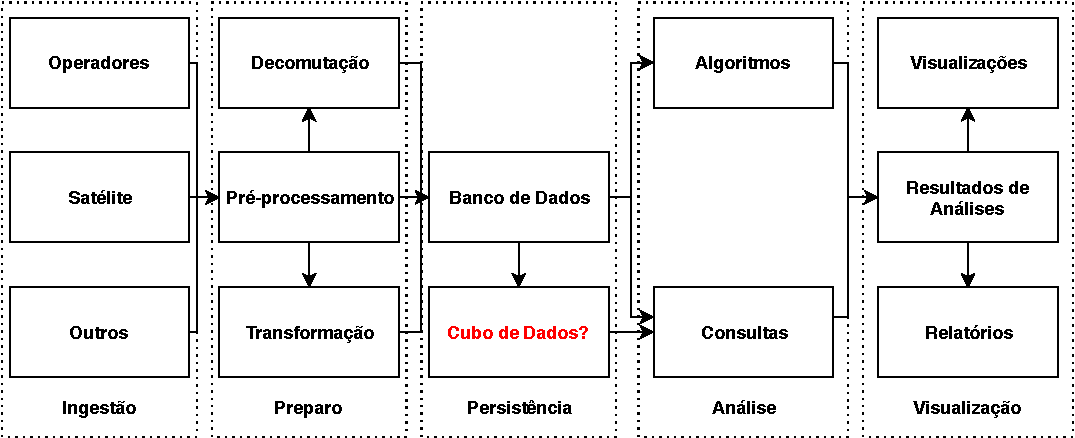
\includegraphics{Figuras/BigDataFlow.pdf}}
	\end{center}
	\vspace{2mm}
	\legenda{}
	\FONTE{Adaptado de~\cite{zhangBigDataFramework2017}}.
	\label{fig:bigdataflow}
\end{figure}

Este fluxo está separado em cinco etapas que vão desde a origem dos dados até o seu resultado de análise, e este trabalho visa apenas mapear qual seria esse fluxo baseado nos trabalhos correlatos, porém adaptado para a realidade do INPE considerando um fluxo ideal.

\section{Arquitetura de um Cubo de Dados}
\label{ch:prop:cubearch}

A figura~\ref{fig:cubearch} demonstra a divisão em 4 camadas de uma estrutura de Cubo de Dados. Essas camadas demonstram tudo o que é necessário para a implementação de um Cubo de Dados, não sendo necessário que uma camada esteja atrelada fortemente a outra.

\begin{figure}[ht]
	\caption{Arquitetura de um cubo de dados}
	\vspace{6mm}
	\begin{center}
		\resizebox{10cm}{!}{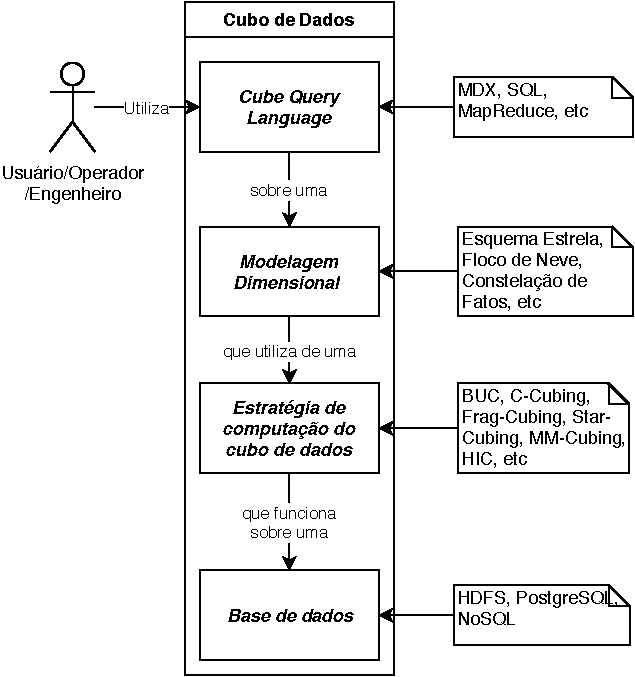
\includegraphics{Figuras/DataCubeArchitecture.pdf}}
	\end{center}
	\vspace{2mm}
	\legenda{}
	\FONTE{Autor (2019)}.
	\label{fig:cubearch}
\end{figure}

Para esta proposta, vamos nos concentrar apenas na proposição de um algoritmo de computação do cubo de dados mais apropriado, utilizando das outras seções quando elas vão se tornando necessárias. Os detalhes, algoritmos e conceitos listados na figura estão majoritariamente descritos na seção~\ref{ch:fun:cube} e não serão repetidos aqui.

Uma informação interessante é que esta estrutura mostra o uso de pelo menos duas linguagens de computação sobre os dados: uma é a Cube Query Language que será utilizada pelo usuário para realizar as operações sobre o cubo (Drill-Down, Roll-up, etc), e outra é a linguagem que será utilizada pelo cubo para realizar essas operações, e elas podem ser independentes, por exemplo, pode-se utilizar SQL extendida com vocabulário de OLAP, porém o algoritmo de cubo de dados internamente pode consultar uma estrutura feita com MapReduce para o cálculo das medidas e das agregações.

Porém, utilizar duas linguagens muito diferentes nesse ponto pode não ser uma boa ideia, pois adicionaria um nível de diferença entre o usuário e os dados.
Caso seja necessário realizar uma consulta OLTP normal, sem o uso do cubo de dados, por exemplo, essa diferença ficaria mais óbvia, por exemplo traduzir uma consulta de SQL para MapReduce não seria muito fácil simplesmente por ter que entender de ambas as linguagens bem para conseguir fazer isso.
Deste modo, é interessante manter a mesma linguagem ao longo da estrutura, apenas alterando nas operações relevantes para o cubo de dados.

Com isso se torna necessário resaltar o último nível, a Base de Dados: a escolha de banco de dados vai impactar como o algoritmo funciona, visto que existem diferentes sistemas de arquivos e como eles são atingidos, bem como o estilo do banco vai mudar como o algoritmo deve gerar o cubo, pois a base pode utilizar diferentes paradigmas de banco de dados~\cite{cuzzocreaDataWarehousingOLAP2013}.

